\section{How to Make Lots of Mistakes} \label{sec:mutate}

An important challenge from~\ref{sec:challenges} is the generation of
mix-typed programs with representative type mistakes. In this section, we
present our generation process and we argue that despite its synthetic
nature it results in a large corpus of programs with type mistakes that
are realistic and diverse.

The starting point for our corpus of programs
is~\citet{gtnffvf-jfp-2019}'s gradual typing benchmark suite. The
benchmark suite consists of fully typed correct programs that are written by different authors
and have been used, maintained and evolved by their authors and others over a
number of years.  They range widely in size, complexity, purpose and
features of Typed Racket they employ.  Furthermore the benchmarks use advanced aspects 
of Typed Racket's type system such as occurrence
typing~\cite{tf-icfp-2010}, types for mutable and immutable data
structures, polymorphic types, types for first-class classes and objects and types for
Racket's numeric tower~\cite{stathff-padl-12}. Without loss of the diversity of the benchmarks,
we select the ten largest in terms of numbers of components (between 6 and 14 components).
These benchmarks also have the most complex dependency graphs and, hence, 
can make the debugging process the hardest for the rational programmer. 
The table in figure~\ref{table:benchmark-descriptions} shows our selection
together with a short description for each benchmark.  


\begin{figure}
\begin{tabular}{p{2cm} | p{10cm} }
  {\bf  name} & {\bf description (author)}  \\

\hline

  \texttt{acquire} & Board game simulation (M. Felleisen)  \\%[1em]


\hline
  \texttt{gregor} & Utilities for calendar dates (J. Zeppieri) \\%[1em]


\hline
  \texttt{kcfa} & Functional implementation of 2CFA for the lambda calculus (M. Might) \\%[1em]


\hline
  \texttt{quadT} & Converter from S-expresion source code to PDF format (M. Butterick)\\%[1em]
    
\hline
  \texttt{quadU} & Converter from S-expresion source code to PDF format  (B. Greenman) \\%[1em]

\hline
  \texttt{snake} & Functional implementation of the  Snake video game (D. Van Horn) \\%[1em]

\hline
  \texttt{suffixtree} & Algorithm for common longest subsequences between strings. (D. Yoo) \\%[1em]

\hline
  \texttt{synth} & Converter of description of notes and drum beats to WAV format (V. St-Amour \& N. Toronto) \\%[1em]

\hline
  \texttt{take5} & Card game simulator (M.Felleisen)  \\%[1em]

\hline
  \texttt{tetris} & Functional implementation of Tetris (D. Van Horn) \\%[1em]


\end{tabular}
  \caption{Benchmarks summary.}
  \label{table:benchmark-descriptions}
\end{figure}

Of course, the gradual typing benchmarks have no mistakes for the rational
programmer to debug. Therefore, we follow
~\citet{lksfd-popl-2020} and we inject bugs with mutation analysis. 
A mutations is a local syntactic change of the code of a program that may
produce a bug. Usually, the outcome of mutating a program
once, dubbed a mutant, can be distinguished from the original program with a test case. 
The better the test suite of a program, the more mutants it can ``kill.''
Thus a big part of research on mutation analysis goes into designing
operations that perform mutations, dubbed mutators, that create mutants 
that are hard to ``kill.'' Unlike the standard mutators, which \citet{lksfd-popl-2020}
use, too, the mutators we need to evaluate the rational programmer have to be
fine-tuned to generate shallow errors. Typed Racket's type system detects 
typos not logical mistakes, and mutators suitable for our purposes
should target the former rather than the latter. 

The table in figure~\ref{table:mutation-ops}  summarizes our mutators. 
For each one, the table provides a short description and an example
mutation it performs. Each mutator is inspired by the more-than-a-decade
long experience of the authors making type errors in Typed Racket. 
Our first ten mutators capture usual common in every type language. 
For instance, position swaps the arguments of a function call.d
The last three mutator target distinguishing features of Typed Racket. 
Specifically, \texttt{arithmetic} may replace a \texttt{+} with a \texttt{-} 
in an attempt to change the type of the result of the arithmetic
operation. In Typed Racket, \texttt{+}'s result is a
\texttt{Positive-Integer} when all arguments are
\texttt{Positive-Integer}. However, the result of \texttt{-} is 
\texttt{Integer}. In the same spirit, \texttt{boolean} aims to take
advantage of Typed Racket's ``truthiness.'' Finally,
\texttt{conditional}'s goal is to confuse occurrence typing.  


\begin{figure}
  \begin{tabular}{p{2.1cm} | p{5cm}  | p{5.5cm} }
    {\bf name} & {\bf description} & {\bf example} \\

 

 
    \texttt{constant}
& Swap a literal constant with another of the same value but different type.
& \texttt{5.6} $\rightarrow$ \texttt{5.6+0.0i} \\
\hline 
    \texttt{deletion}
    & Deletes the result expression of a \texttt{begin} or \texttt{begin0}
    sequence.
    & \texttt{(begin x y z)} $\rightarrow$ \texttt{(begin x y)} \\
\hline


 \texttt{id}
 & Swaps a use of a top-level identifier defined with with another defined
 in the same module.
 &\texttt{(f ...)} $\rightarrow$ \texttt{(g ...)}\\
\hline


    \texttt{list}
    & Swap \texttt{car} and \texttt{cdr}.
    & \texttt{car} $\rightarrow$ \texttt{cdr} \\
 \hline    



   \texttt{position}
 & Swap the position of subexpressions.
  &  \begin{tabular}[t]{@{}l}
     \texttt{(f a 42 "b" 0)}\\
       $\rightarrow$\\ 
      \texttt{(f a 42 0 "b")}
    \end{tabular}\\
\hline 

\texttt{class:init}
  & Swap default values of class fields.
   &  \begin{tabular}[t]{@{}l}
     \texttt{(class object\%}\\
     \texttt{\,\,(field [a 5] [b "hello"]))}\\
       $\rightarrow$\\ 
      \texttt{(class object\%}\\
     \texttt{\,\,(field [a "hello"] [b 5]))}\\
    \end{tabular}\\
\hline 


\texttt{class:method}
 & Add an extra trivial public method to a class.
 &  \begin{tabular}[t]{@{}l}
   \texttt{(class object\%  ...)}\\
       $\rightarrow$\\ 
     \texttt{(class object\%}\\
     \texttt{\,\,(define/public (extra x) x)}\\
     \texttt{\,\,...)}
    \end{tabular}\\
\hline

\texttt{class:parent}
    & Replace the parent of classes with \texttt{object\%}.
    &  \begin{tabular}[t]{@{}l}
     \texttt{(class foo\% ...)}\\
       $\rightarrow$\\ 
      \texttt{(class object\% ...)}\\
    \end{tabular}\\
\hline     



\texttt{class:public}
    & Make a public method private and vice versa.
    & 
    \begin{tabular}[t]{@{}l}
      \texttt{(class object\%}\\
        \texttt{\,\,(define/public (m x) x))}\\
       $\rightarrow$\\ 
      \texttt{(class object\%}\\
        \texttt{\,\,(define/private (m x) x))}\\
    \end{tabular}\\
\hline 

 \texttt{class:super}
    & Remove \texttt{super-new} calls from class definitions.
    &  \begin{tabular}[t]{@{}l}
      \texttt{(class object\% (super-new))}\\
       $\rightarrow$\\ 
      \texttt{(class object\% (void))}\\
    \end{tabular}\\
\hline

 
 

\texttt{arithmetic} 
& Swap an arithmetic operator with another one of the same (or greater)
    arity and a possibly different result type. 
    & \texttt{+} $\rightarrow$ \texttt{-} \\
\hline   

\texttt{boolean} 
& Swap \texttt{and} and \texttt{or}. Due to Racket's truthiness it
    possibly changes the type of the operation's result. 
& \texttt{and} $\rightarrow$ \texttt{or} \\

\hline 


\texttt{conditional}
    & Negate conditional test expressions.
    &  \begin{tabular}[t]{@{}l}
      \texttt{(cond [(= x 0) 42] ...)}\\ 
       $\rightarrow$\\ 
      \texttt{(cond [(not (= x 0)) 42] ...)}
    \end{tabular}\\
\hline 

   

\end{tabular}
  \caption{Summary of mutators.}
  \label{table:mutation-ops}
\end{figure}

An effective set of mutators for type errors should be able to generate
a large number of ill-typed programs. Hence, to validate that our experience 
with Typed Racket translates to effective mutators, we analyze the
 mutants of our ten benchmarks. Figure~\ref{fig:mutators-static-hit} shows
 the results. For each benchmark, our mutators generate between 156 and
 18165 ill-typed mutants. Most importantly the collective success rate of
 the mutators  per benchmark, i.e., the percentage of ill-typed mutants 
 over the number of mutants, ranges between 53\% (\texttt{tetris})
 and 95\% (\texttt{kCFA}). Finally, the figure depicts the individual success rate 
 of mutators per benchmark which reveals that there is at
 least one benchmark where each mutator performs well
 (>90\%).

\begin{figure}
  \centering
  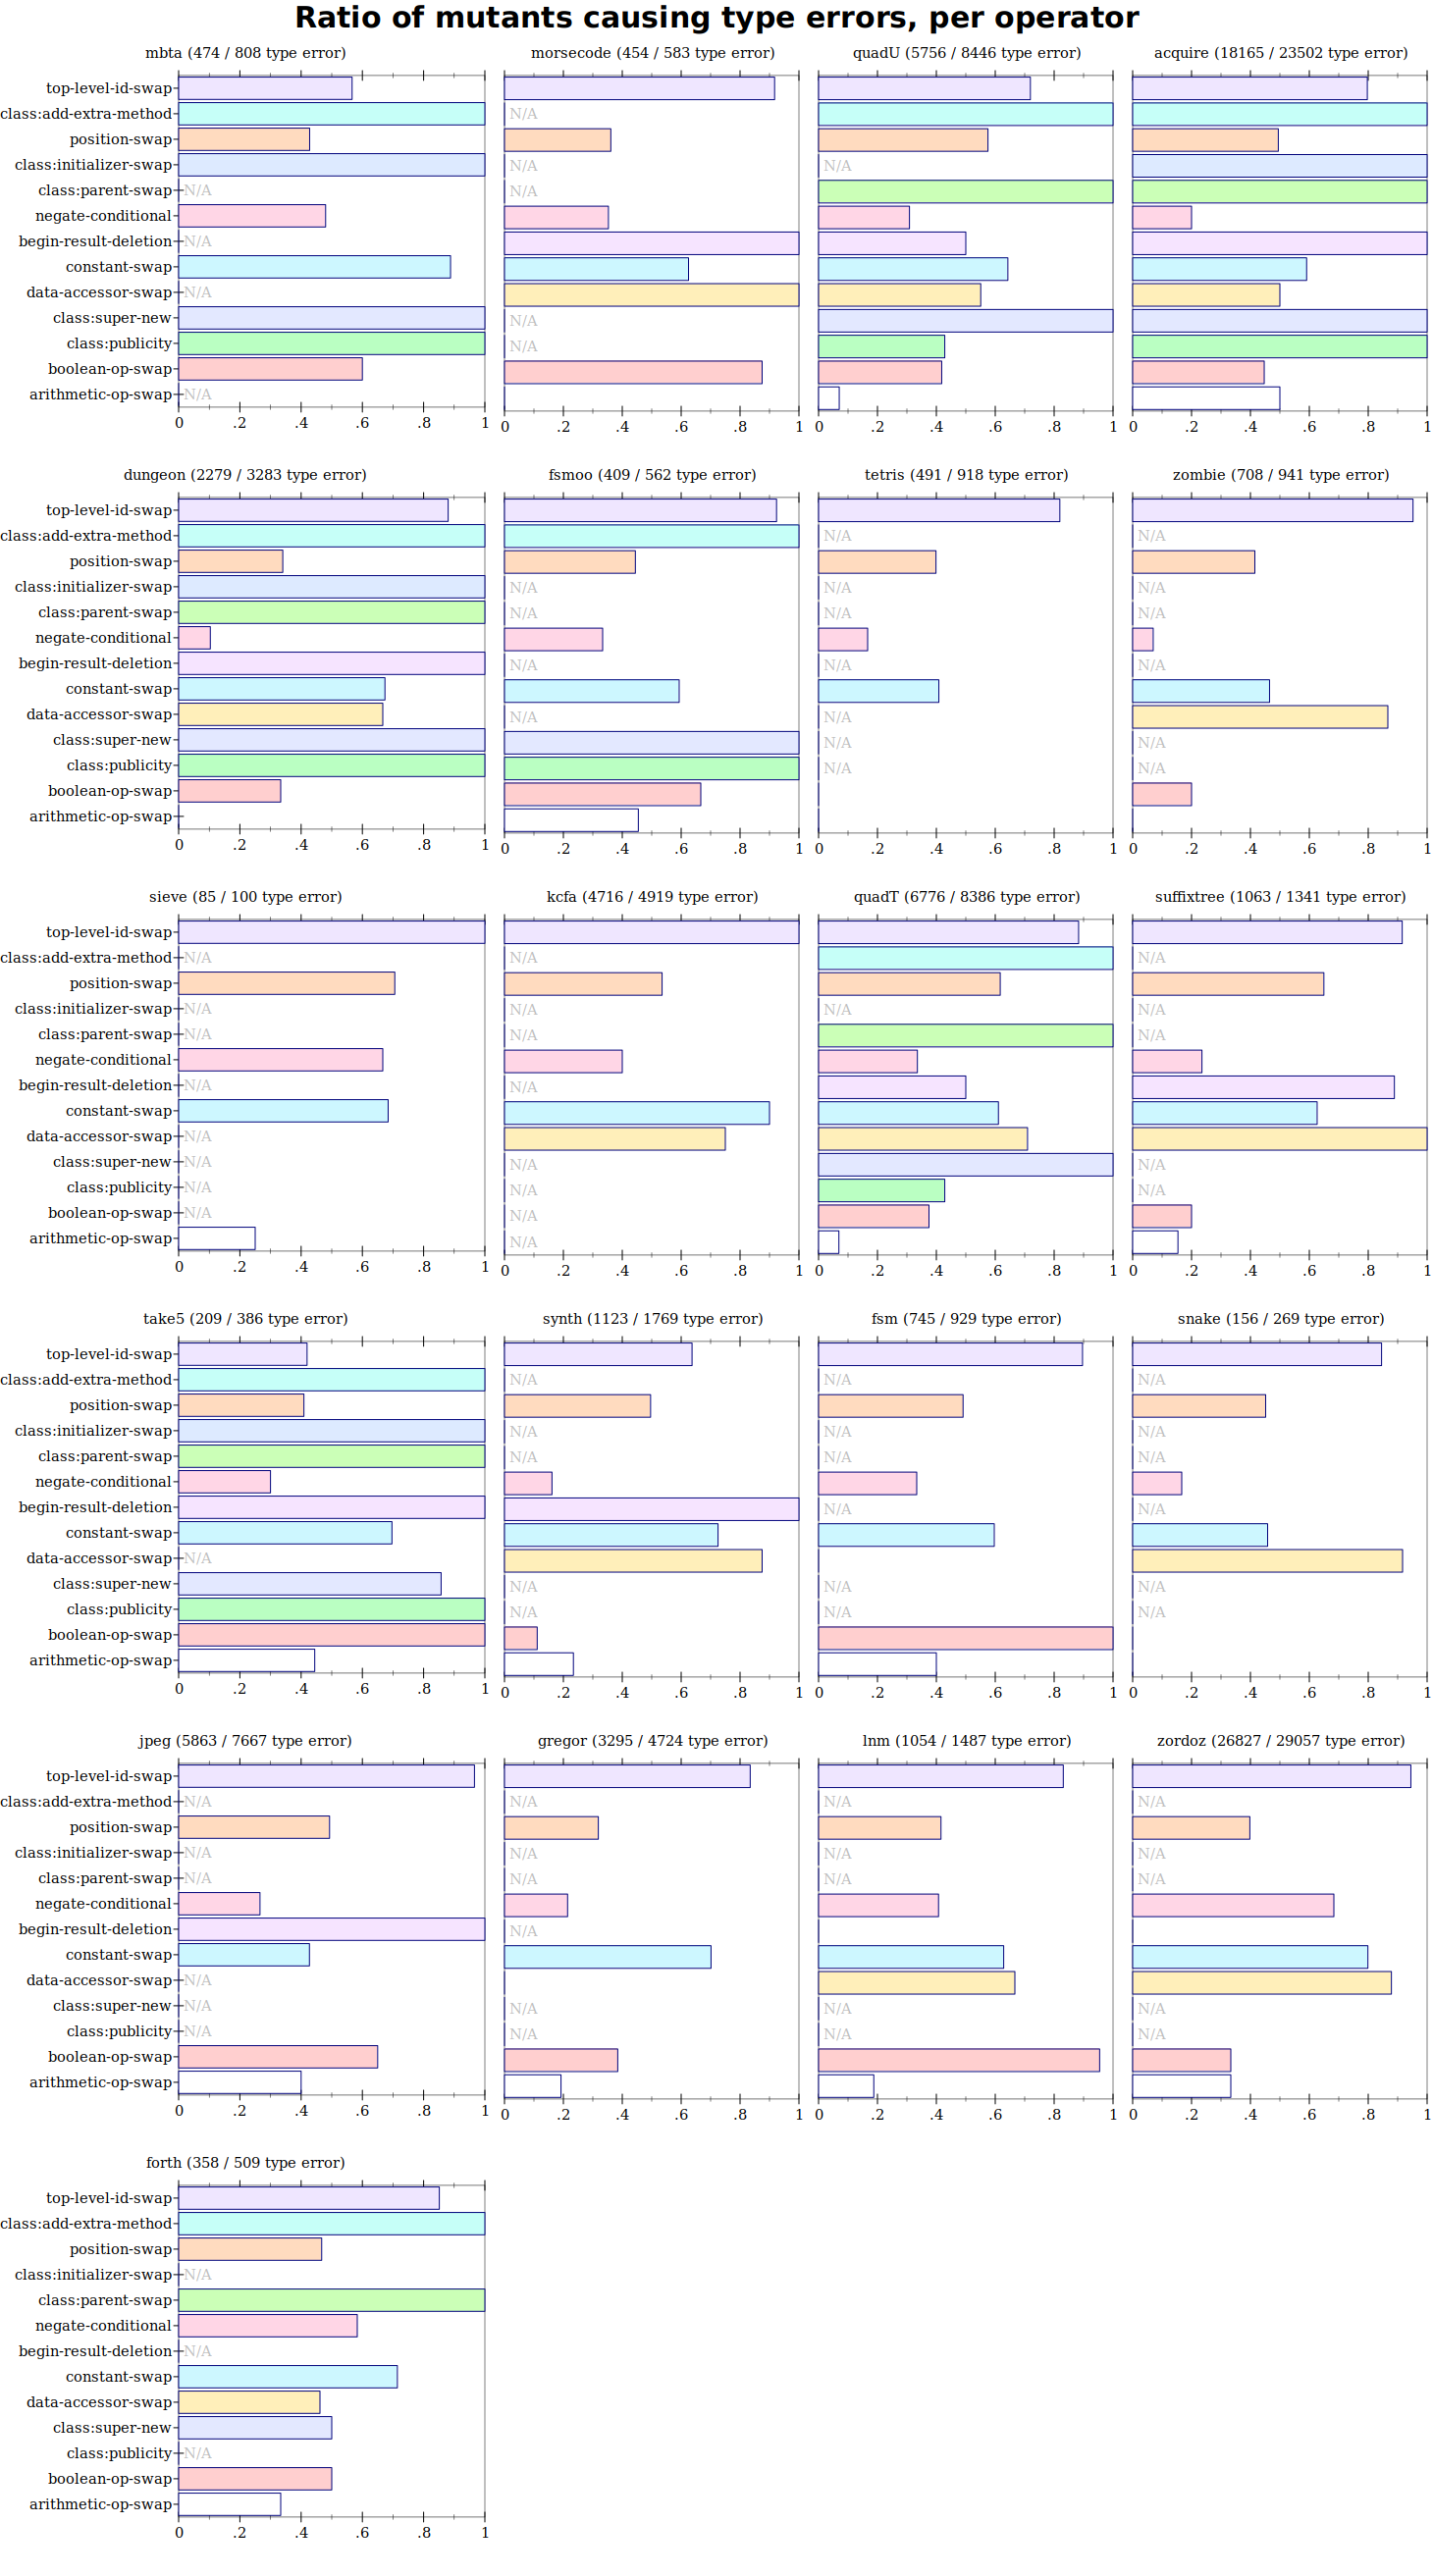
\includegraphics[width=\textwidth]{./plots/code-hit-ratios}
  \caption{Success rate of mutators (the percentage of ill-typed mutants 
  over the number of mutants)}
  \label{fig:mutators-static-hit}
\end{figure}

So far we have established that our mutators and~\citet{gtnffvf-jfp-2019}'s 
benchmarks are sufficient to create a large number of realistic ill-typed Type Racket
programs. However, in an ill-typed program with correct types, like
in our case, it is trivial to figure out which component contains the bug.
It is the component that doesn't type check. Thus the ill-typed mutants
do not offer an interesting setting to try out the debugging abilities of
rational programmers. That said, we can derive interesting debugging
scenarios by removing type specifications from some of the components of
the benchmarks. The resulting mix-typed programs may be well-typed and when
run may raise a type error. Section~\ref{sec:rational} explains how we can
explore the space of debugging scenarios in a principled manner. As a
final remark in this section, with the data from
figure~\ref{fig:mutators-runtime-hit}, we verify  that in each of the three semantics
we target, between 25\% and
90\% of the ill-typed mutants each mutator generates give rise to at least one interesting debugging scenario.


\begin{figure}
  \centering
  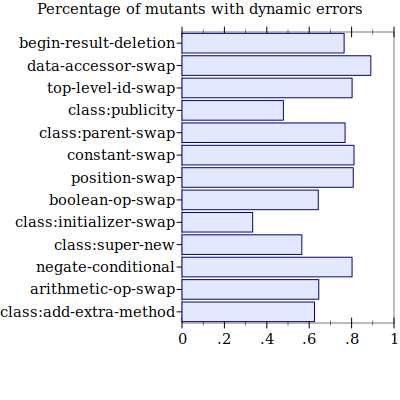
\includegraphics[width=\textwidth]{./plots/code-dynamic-error}
  \caption{}
  \label{fig:mutators-runtime-hit}
\end{figure}

